\documentclass[10pt]{article}
\usepackage[pdftex]{graphicx, color}
\usepackage{listings}

\usepackage{tikz}
\usetikzlibrary{automata,positioning}

\headheight 8pt \headsep 20pt \footskip 30pt
\textheight 9in \textwidth 6.5in
\oddsidemargin 0in \evensidemargin 0in
\topmargin -.35in

\newcommand {\pts}[1]{({\bf #1 pts})}   
\lstset{basicstyle=\small\ttfamily,breaklines=true}

\begin{document}
\begin{center}
\Large CS131 Compilers: Writing Assignment 1\\Due Tuesday, March 9, 2017 at 8:15am
\end{center}

\begin{center}
%% Change this:
\LARGE Name - ID
\end{center}


This assignment asks you to prepare written answers to questions on
regular languages, finite automata, and lexical analysis.  Each of the
questions has a short answer.  You may discuss this assignment with
other students and work on the problems together.  However, your
write-up should be your own individual work and you should indicate in your submission who you worked
with, if applicable.  Written assignments are turned in at the start of lecture.
You should use the Latex template provided at the course web site to write your solution and use the \emph{tikz} package to draw
automata.

\begin{center}
%% Change this:
I worked with:
\end{center}

\begin{enumerate}
  \item \pts{$2\times 3=6$} For each of the follow prompts, write any non-empty sentence:
  \begin{enumerate}
           \item Name one reason why you would like to learn in this class.
            

              \textbf{I want to learn how to write a compiler.}
              %% Your answer here
            

           \item Write a question you would like the professor to answer ¡ª on any topic, from personal opinions to the class material.
            

              \textbf{Why don't we write a compiler without tools?}
              %% Your answer here
            

           \item What do you expect from this class.
            

             \textbf{ Learn very cool things.}
              %% Your answer here
            

  \end{enumerate}
  %
  \item \pts{$2\times 4=8$} Write regular expressions for the following languages over the alphabet $\Sigma=\{0,1\}$:
 \begin{enumerate}
           \item $L_1$: The set of all finite strings containing at least three $1's$.
            \[
             [01]^{*}1[01]^{*}1[01]^{*}1[01]^{*}
            \]
           \item $L_2$: The set of all finite strings containing at most two $0's$.
            \[
             [1]^{*}[0]?[1]^{*}[0]?[1]^{*}
            \]
            %% Your answer here
           \item $L_3$: The set of all finite strings containing at most two $0's$ and at least three $1's$.
            \\
            \\
           { | is \|}
            
            ([1]*0[1]*111|[1]*10[1]*11|[1]*11*0[1]*1|111[1]*0[1]*\\|[1]*00[1]*111|[1]*100[1]*11|[1]*11*00[1]*1|111[1]*00[1]*|[1]*01[1]*011[1]*\\|[1]*011[1]*01[1]*|[1]*0111[1]*0[1]*|[1]*10[1]*10[1]*1|[1]*10[1]*110[1]*|11[1]*0[1]*10[1]*)
            \\
            \\
           \item $L_4$: The set of all finite strings containing at least three $1's$, but no two $1's$ appear convectively.
            \[
            [0]^{*}1[0]^{+}1([0]^{+}1[0]^{*})^{+}
            %% Your answer here
            \]
   \end{enumerate}
   This example illustrates that regular languages are closed under intersection. Note that
   $L_3=L_1\cap L_2$.

  \newpage
   \item \pts{$2\times 4=8$} Draw DFA's for each of the languages $L_1$, $L_2$, $L_3$ and $L_4$ from Question 1.
  \begin{enumerate}
    \item $L_1$.
    \\
    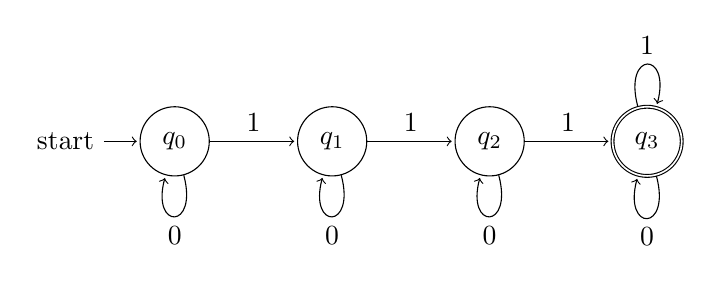
\begin{tikzpicture}[shorten >=1pt,node distance=2cm,on grid,auto]
        \node[state,initial] (q_0)   {$q_0$};
        \node[state] (q_1) [right=of q_0] {$q_1$};
        \node[state] (q_2) [right=of q_1] {$q_2$};
        \node[state,accepting](q_3) [right=of q_2] {$q_3$};
        \path[->]
        (q_0) edge [loop below] node {0} ()
              edge  node {1} (q_1)
        (q_1) edge [loop below] node {0} ()
              edge  node {1} (q_2)
        (q_2) edge [loop below] node {0} ()
              edge  node {1} (q_3)
        (q_3) edge [loop below] node {0} ()
              edge [loop above] node {1} ();
        %% Your answer here
    \end{tikzpicture}
    \item $L_2$.
    \\
    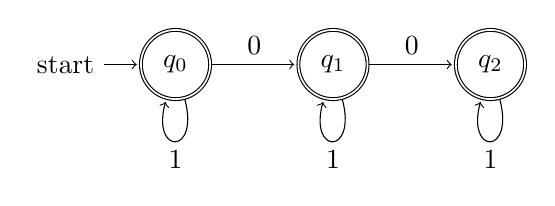
\begin{tikzpicture}[shorten >=1pt,node distance=2cm,on grid,auto]
        \node[state,initial,accepting]   (q_0)   {$q_0$};
        \node[state,accepting] (q_1) [right=of q_0] {$q_1$};
        \node[state,accepting] (q_2) [right=of q_1] {$q_2$};
        \path[->]
        (q_0) edge [loop below] node {1} ()
              edge  node {0} (q_1)
        (q_1) edge [loop below] node {1} ()
              edge  node {0} (q_2)
        (q_2) edge [loop below] node {1} ();
        %% Your answer here
    \end{tikzpicture}
    \item $L_3$.
    \\
    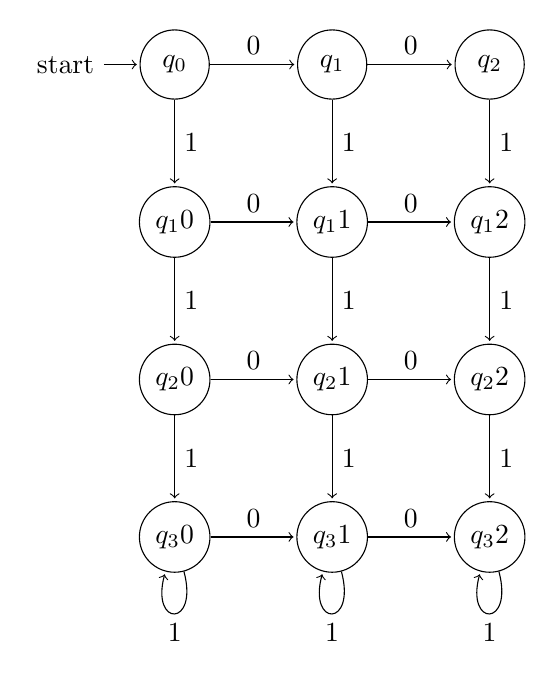
\begin{tikzpicture}[shorten >=1pt,node distance=2cm,on grid,auto]
        \node[state,initial]   (q_0)   {$q_0$};
        \node[state]   (q_1) [right=of q_0]  {$q_1$};
        \node[state]   (q_2) [right=of q_1]  {$q_2$};
        \node[state]   (q_10) [below=of q_0]  {$q_10$};
        \node[state]   (q_11) [right=of q_10]  {$q_11$};
        \node[state]   (q_12) [right=of q_11]  {$q_12$};
        \node[state]   (q_20) [below=of q_10]  {$q_20$};
        \node[state]   (q_21) [right=of q_20]  {$q_21$};
        \node[state]   (q_22) [right=of q_21]  {$q_22$};
        \node[state]   (q_30) [below=of q_20]  {$q_30$};
        \node[state]   (q_31) [right=of q_30]  {$q_31$};
        \node[state]   (q_32) [right=of q_31]  {$q_32$};
        \path[->]
        (q_0) edge node {0} (q_1) 
              edge node {1} (q_10) 
        (q_1) edge node {0} (q_2) 
              edge node {1} (q_11) 
        (q_2) edge node {1} (q_12)
        
        (q_10) edge node {0} (q_11) 
               edge node {1} (q_20)
        (q_11) edge node {0} (q_12)
               edge node {1} (q_21) 
        (q_12) edge node {1} (q_22) 
        
        (q_20) edge node {0} (q_21)
               edge node {1} (q_30)
        (q_21) edge node {0} (q_22)
               edge node {1} (q_31)
        (q_22) edge node {1} (q_32) 
        
        (q_30) edge node {0} (q_31)
               edge [loop below] node {1} () 
        (q_31) edge node {0} (q_32) 
               edge [loop below] node {1} () 
        (q_32) edge [loop below] node {1} (q_32) ;
        %% Your answer here
    \end{tikzpicture}
     \item $L_4$.
    \\
    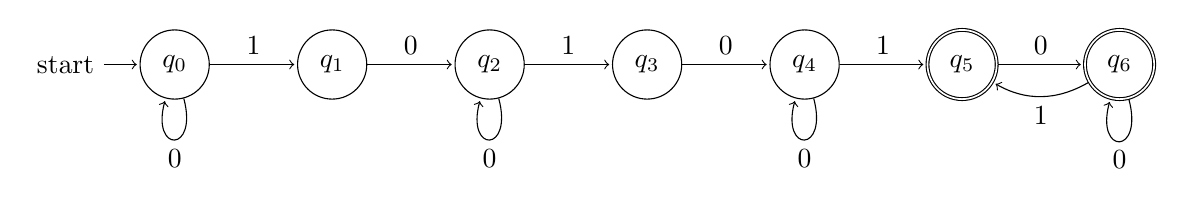
\begin{tikzpicture}[shorten >=1pt,node distance=2cm,on grid,auto]
        \node[state,initial] (q_0)   {$q_0$};
        \node[state] (q_1) [right=of q_0] {$q_1$};
        \node[state] (q_2) [right=of q_1] {$q_2$};
        \node[state] (q_3) [right=of q_2] {$q_3$};
        \node[state] (q_4) [right=of q_3] {$q_4$};
        \node[state,accepting] (q_5) [right=of q_4] {$q_5$};
        \node[state,accepting] (q_6) [right=of q_5] {$q_6$};
        \path[->]
        (q_0) edge [loop below] node {0} ()
              edge  node {1} (q_1)
        (q_1) edge  node {0} (q_2)
        (q_2) edge [loop below] node {0} ()
              edge  node {1} (q_3)
        (q_3) edge  node {0} (q_4)
        (q_4) edge [loop below] node {0} ()
              edge  node {1} (q_5)
        (q_5) edge  node {0} (q_6)
        (q_6) edge [loop below] node {0} ()
              edge [bend left] node {1} (q_5);
        %% Your answer here
    \end{tikzpicture}
  \end{enumerate}

   \newpage


  \item \pts{$5\times 3=15$} Using the techniques covered in class, transform the following NFAs with $\epsilon$-transitions over the given alphabet $\Sigma$ into DFAs. Note that a DFA must have a transition defined for every state and symbol pair, whereas a NFA need not. You must take this fact into account for your transformations. Hint: Is there a subset of states the NFA transitions to when fed a symbol for which the set of current states has no explicit transition?

  \begin{enumerate}
    \item Original NFA, $\Sigma = \{a, b, c\}$:
    \\
    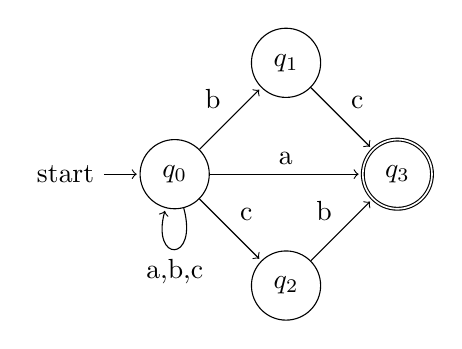
\begin{tikzpicture}[shorten >=1pt,node distance=2cm,on grid,auto]
        \node[state,initial] (q_0)   {$q_0$};
        \node[state] (q_1) [above right=of q_0] {$q_1$};
        \node[state] (q_2) [below right=of q_0] {$q_2$};
        \node[state,accepting](q_3) [below right=of q_1] {$q_3$};
        \path[->]
        (q_0) edge [loop below] node {a,b,c} ()
              edge  node  [above] {a} (q_3)
              edge  node  {b} (q_1)
              edge  node  {c} (q_2)
        (q_1) edge  node  {c} (q_3)
        (q_2) edge  node  {b} (q_3);
    \end{tikzpicture}
    \\
    DFA:
    
    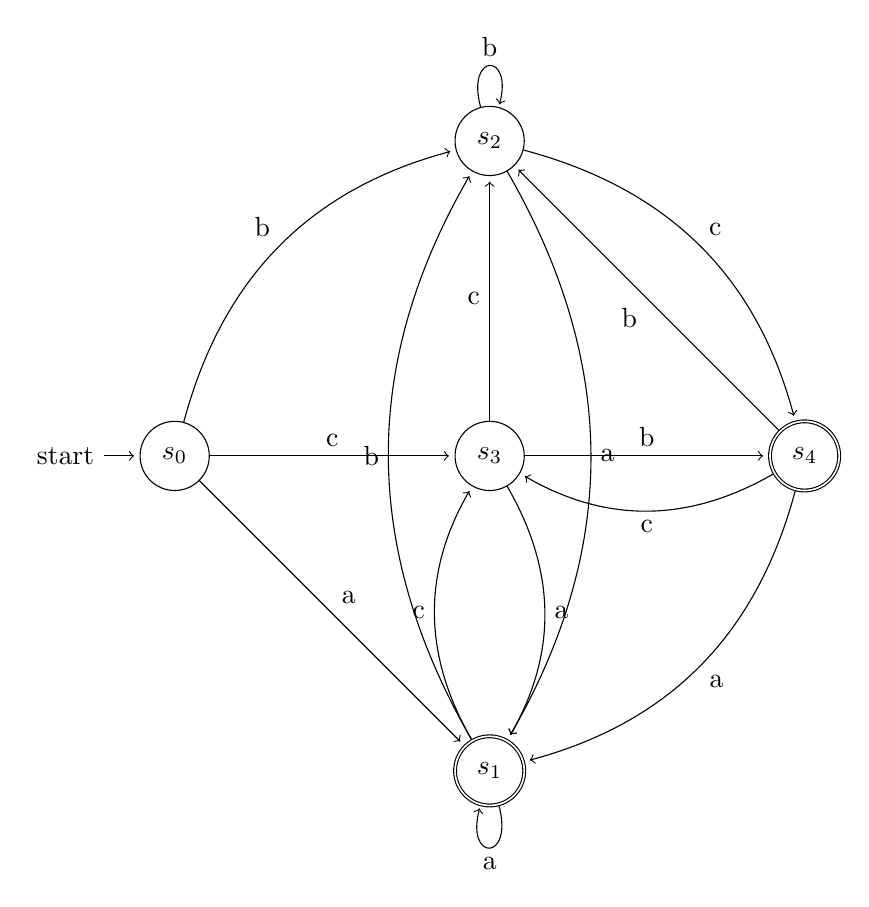
\begin{tikzpicture}[shorten >=2pt,node distance=4cm,on grid,auto]
        \node[state,initial] (s_0)   {$s_0$};
        \node[state] (s_3) [right=of s_0] {$s_3$};
        \node[state,accepting] (s_1) [below=of s_3] {$s_1$};
        \node[state] (s_2) [above=of s_3] {$s_2$};
        \node[state,accepting] (s_4) [right=of s_3] {$s_4$};
        \path[->]
        (s_0) edge  node  {a} (s_1)
              edge [bend left] node  {b} (s_2)
              edge  node  {c} (s_3)
        (s_1) edge [loop below] node  {a} ()
              edge [bend left] node  {b} (s_2)
              edge [bend left] node  {c} (s_3)
        (s_2) edge [bend left] node  {a} (s_1)
              edge [loop above] node  {b} ()
              edge [bend left] node  {c} (s_4)
        (s_3) edge [bend left] node  {a} (s_1)
              edge  node  {b} (s_4)
              edge  node  {c} (s_2)
        (s_4) edge [bend left] node  {a} (s_1)
              edge  node  {b} (s_2)
              edge [bend left] node  {c} (s_3);
    \end{tikzpicture}

    \item Original NFA, $\Sigma = \{a, b, c\}$:
    \\
    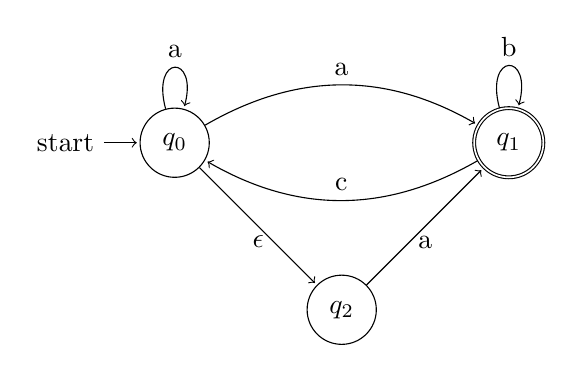
\begin{tikzpicture}[shorten >=1pt,node distance=3cm,on grid,auto]
        \node[state,initial] (q_0)   {$q_0$};
        \node[state] (q_2) [below right=of q_0] {$q_2$};
        \node[state,accepting] (q_1) [above right=of q_2] {$q_1$};
        \path[->]
        (q_0) edge [loop above] node {a} ()
              edge [bend left] node  {a} (q_1)
              edge  node [below] {$\epsilon$} (q_2)
        (q_1) edge [loop above] node {b} ()
              edge [bend left] node [above] {c} (q_0)
        (q_2) edge node [below] {a} (q_1);
    \end{tikzpicture}
    \\
    \\
    \\
    DFA:
    \\
    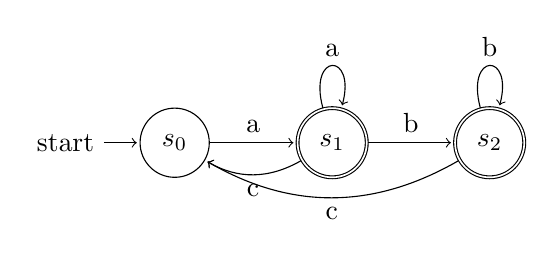
\begin{tikzpicture}[shorten >=1pt,node distance=2cm,on grid,auto]
        \node[state,initial] (s_0)   {$s_0$};
        \node[state,accepting] (s_1) [right=of s_0]  {$s_1$};
        \node[state,accepting] (s_2) [right=of s_1]  {$s_2$};
        \path[->]
        (s_0)  edge node {a} (s_1)
        (s_1)  edge [loop above] node {a} (s_1)
               edge node {b} (s_2)
               edge [bend left] node {c} (s_0)
        (s_2)  edge [bend left] node {c} (s_0)
               edge [loop above] node {b} (s_2);
        %% Your answer here
    \end{tikzpicture}
    \item Original NFA, $\Sigma = \{a, b,c\}$:
    \\
    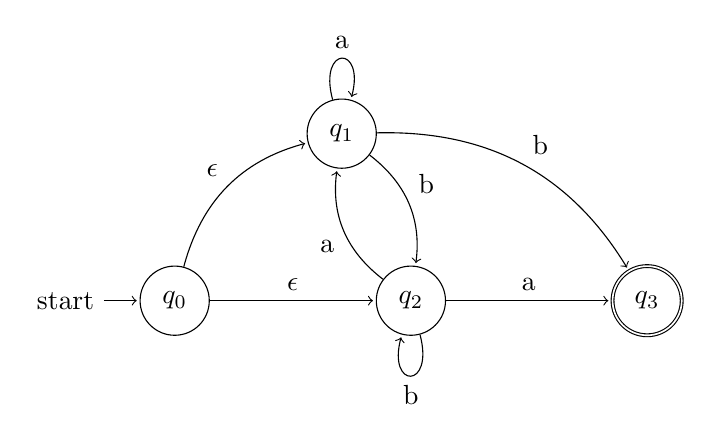
\begin{tikzpicture}[shorten >=1pt,node distance=3cm,on grid,auto]
        \node[state,initial] (q_0)   {$q_0$};
        \node[state] (q_1) [above right=of q_0] {$q_1$};
        \node[state] (q_2) [right=of q_0] {$q_2$};
        \node[state,accepting] (q_3) [right=of q_2] {$q_3$};
        \path[->]
        (q_0) edge [bend left] node  {$\epsilon$} (q_1)
              edge node  {$\epsilon$} (q_2)
        (q_1) edge [loop above] node {a} ()
              edge [bend left] node {b} (q_3)
              edge [bend left] node {b} (q_2)
        (q_2) edge [loop below] node {b} ()
              edge node {a} (q_3)
              edge [bend left] node {a} (q_1);
    \end{tikzpicture}
    \\
    DFA:
    \\E1=E2
    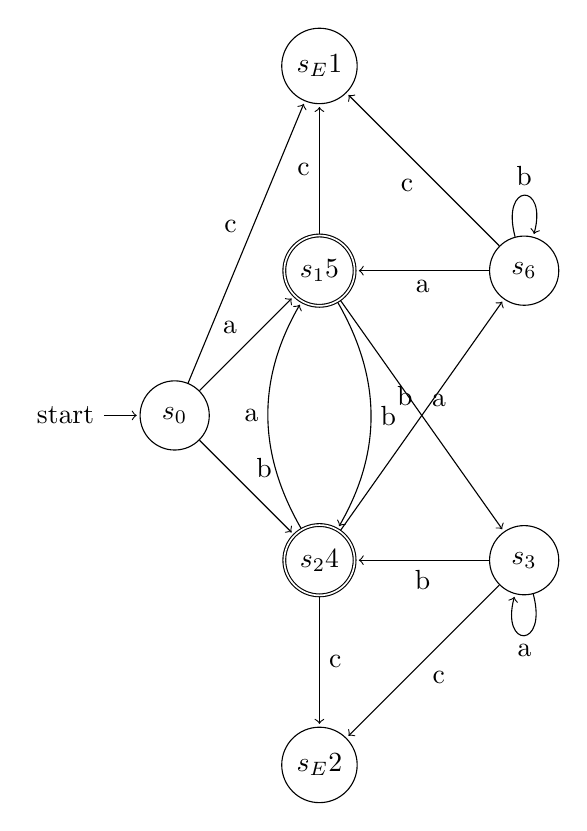
\begin{tikzpicture}[shorten >=1pt,node distance=2.6cm,on grid,auto]
        \node[state,initial] (s_0)   {$s_0$};
        \node[state,accepting] (s_15) [above right=of s_0] {$s_15$};
        \node[state,accepting] (s_24) [below right=of s_0] {$s_24$};
        \node[state] (s_3) [right=of s_24] {$s_3$};
        \node[state] (s_6) [right=of s_15] {$s_6$};
        \node[state] (s_E1) [above=of s_15] {$s_E1$};
        \node[state] (s_E2) [below=of s_24] {$s_E2$};
        \path[->]
        (s_0) edge node  {a} (s_15)
              edge node  {b} (s_24)
              edge node  {c} (s_E1)
        (s_15) edge node {a} (s_3)
               edge [bend left] node {b} (s_24)
               edge node  {c} (s_E1)
        (s_24) edge node {b} (s_6)
               edge [bend left] node {a} (s_15)
               edge node  {c} (s_E2)
        (s_3)  edge [loop below] node {a} (s_3)
               edge node {b} (s_24)
               edge node  {c} (s_E2)
        (s_6)  edge [loop above] node {b} (s_6)
               edge node {a} (s_15)
               edge node  {c} (s_E1);
        %% Your answer here
    \end{tikzpicture}
  \end{enumerate}

   \newpage
  \item \pts{$13$} Draw the NFA for the set of all strings over the alphabet $\Sigma = \{a,b\}$, where either $a$ occurs
an odd number of times and each of pair of a's is separated by exactly $2n+2$ consecutive b's (for some $n \geq 0$), or $b$ occurs
an even number of times and each of pair of relative consecutive b's is separated by exactly $2m+1$ consecutive a's (for some $m \geq 0$).
Examples of strings that should be accepted by this NFA: abbabbbba, babaaabaaaaab.
Examples of strings that should \textbf{not} be accepted: ababb, abbbabba.
    \\
    \\
    \begin{tikzpicture}[shorten >=1pt,node distance=2cm,on grid,auto]
        \node[state,initial]   (q_0)   {$q_0$};
        \node[state] (q_1) [above=of q_0] {$q_1$};
        \node[state] (q_2) [above,right=of q_1] {$q_2$};
        \node[state] (q_4) [above,right=of q_3] {$q_4$};
        \node[state] (q_6) [above,right=of q_2] {$q_6$};
        \node[state] (q_3) [above,right=of q_6] {$q_3$};
        \node[state] (q_5) [below=of q_0] {$q_5$};
        \node[state] (q_7) [below,right=of q_5] {$q_7$};
        \node[state] (q_8) [below,right=of q_7] {$q_8$};
        \node[state] (q_9) [below,right=of q_8] {$q_9$};
        \node[state,accepting] (q_10) [right=of q_0] {$q_10$};
        \path[->]
        (q_0) edge  node {$\epsilon$} (q_1)
              edge  node {$\epsilon$} (q_5)
              edge  node [bend left] {$\epsilon$} (q_10)
        (q_1) edge  node {a} (q_2)
        (q_2) edge  node {b} (q_6)
              edge  node {$\epsilon$} (q_10)
        (q_6) edge  node {b} (q_3)
        (q_3) edge [bend left] node {$\epsilon$} (q_2)
              edge  node {a} (q_4)
        (q_4) edge [bend left] node {$\epsilon$} (q_2)
              edge node {$\epsilon$} (q_10)
        (q_5) edge  node {b} (q_7)
        (q_7) edge  node {a} (q_8)
              edge  node {$\epsilon$} (q_10)
        (q_8) edge [bend left] node {a} (q_7)
              edge  node {b} (q_9)
        (q_9) edge [bend left] node {a} (q_7)
              edge node {$\epsilon$} (q_10);
    \end{tikzpicture}

  \newpage
   \item Consider the following tokens and their associated regular expressions, given as a \textbf{flex} scanner specification:

  \begin{lstlisting}
    %%
    (if)                    {printf("IF");}
    [0-9]+                  {printf("NUM");}
    [a-zA-Z0-9]+            {printf("ID");}
    [ ]                     {}
  \end{lstlisting}

  Give an input to this scanner such that the output string is $\tt (IF^{\rm 2} ID^{\rm 3} NUM^{\rm 2})^{\rm 2}$, where $\tt A^i$ denotes {\tt A} repeated {\tt i} times.   (And, of course, the parentheses are not part of the output.)  You may use similar shorthand notation in your answer.

        if if id id id 1 2 3 if if id id id 1 2 3
      %% Your answer here


  \newpage
  \item Draw the minimal DFA of the DFA constructed in Question 4(c).
   \\
    \\
    \\E1=E2
    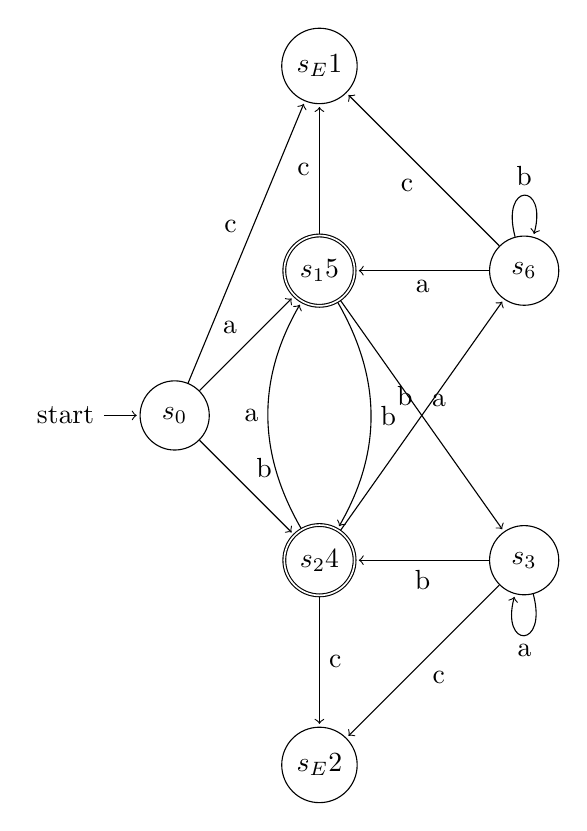
\begin{tikzpicture}[shorten >=1pt,node distance=2.6cm,on grid,auto]
        \node[state,initial] (s_0)   {$s_0$};
        \node[state,accepting] (s_15) [above right=of s_0] {$s_15$};
        \node[state,accepting] (s_24) [below right=of s_0] {$s_24$};
        \node[state] (s_3) [right=of s_24] {$s_3$};
        \node[state] (s_6) [right=of s_15] {$s_6$};
        \node[state] (s_E1) [above=of s_15] {$s_E1$};
        \node[state] (s_E2) [below=of s_24] {$s_E2$};
        \path[->]
        (s_0) edge node  {a} (s_15)
              edge node  {b} (s_24)
              edge node  {c} (s_E1)
        (s_15) edge node {a} (s_3)
               edge [bend left] node {b} (s_24)
               edge node  {c} (s_E1)
        (s_24) edge node {b} (s_6)
               edge [bend left] node {a} (s_15)
               edge node  {c} (s_E2)
        (s_3)  edge [loop below] node {a} (s_3)
               edge node {b} (s_24)
               edge node  {c} (s_E2)
        (s_6)  edge [loop above] node {b} (s_6)
               edge node {a} (s_15)
               edge node  {c} (s_E1);
        %% Your answer here
    \end{tikzpicture}

\end{enumerate}
\end{document}

